\section{Implementation}
The existing implementation of the \gls{sdr} workflow for high energy
accelerator-driven nuclear systems determine the nuclear
inventory changes at the resolution of a geometric cell. This workflow uses a
specialized tally during the first transport step to collect the nuclear
inventory changes. This current workflow can be seen in Figure
\ref{fig:cell_rnucs}.
\begin{figure}[H]
	\centering
	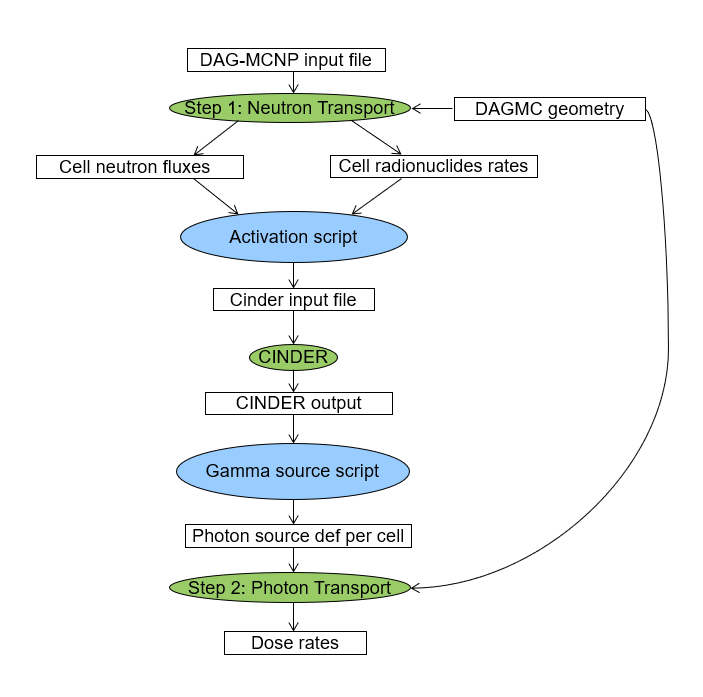
\includegraphics[scale=0.4]{../figs/rnucs_r2s.png}
	\caption{Cell based \gls{sdr}-rnucs Workflow}
	\label{fig:cell_rnucs}
\end{figure}
%
This work extends the specialized tally to function at the resolution of an
arbitrary Cartesian mesh, enabling a higher fidelity \gls{sdr} for high energy
accelerator-driven nuclear systems. An overview of the new workflow can be seen
in Figure  \ref{fig:mesh_rnucs}.
Implementation of the mesh \gls{sdr}-rnucs workflow required changes to
various parts of the workflow as will be described in the following sections.
\begin{figure}[H]
	\centering
	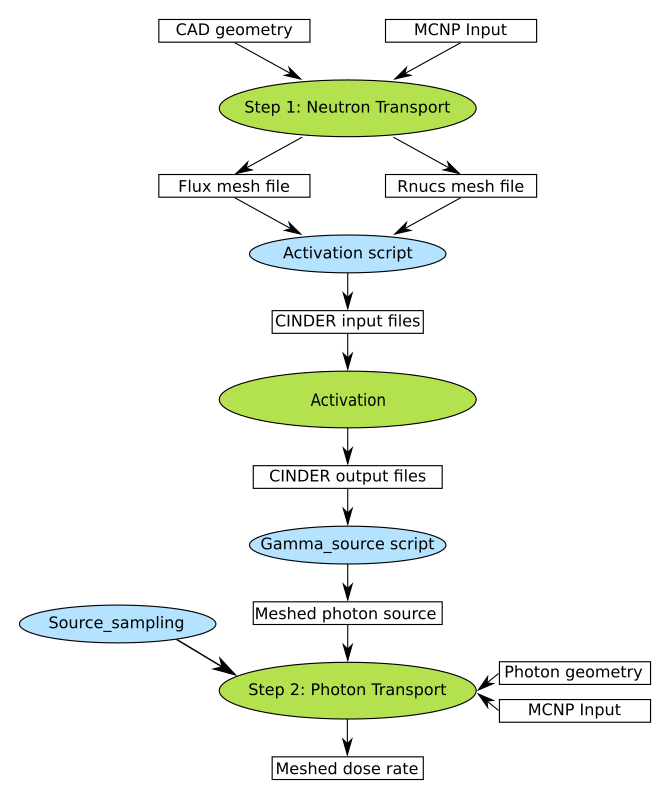
\includegraphics[scale=0.5]{../figs/rnucs_mesh.png}
	\caption{Mesh based \gls{sdr}-rnucs Workflow}
	\label{fig:mesh_rnucs}
\end{figure}
%
%
\subsection{MCNP Patch}
The first step in the \gls{sdr} workflow is a transport step to collect
fluxes, for neutrons of energy up to 20 MeV, and radionuclide information, from
neutron interactions higher than 20 MeV. For this implementation, all the
transport steps are done using the \gls{mcnp} software.\\
First a \gls{dag} and rnucs patch is applied to modify the source \gls{mcnp}
code to be able to use \gls{cad} geometries and the specialized tally,
\textit{rnucs}. Changes to the specialized tally, \textit{rnucs}, were made in
order to collect radionuclide information on an arbitrary Cartesian mesh. These
changes are made directly in the \gls{mcnp} source code, so a patch was created
to apply these changes. This patch should be applied after applying the
\gls{dag}-rnucs patch. These changes have been made for \gls{mcnp}6.1, but can
be expanded to other versions of \gls{mcnp} in the future.
This workflow now outputs a new file called \textit{r\_mesh} which contains the
radionuclide production and destruction per voxel in a mesh. This files was
modeled after a \textit{meshtal} file.
%
\subsubsection{Data Structure}
The extension of the \textit{rnucs} tally comes  with some shortcomings that
should be addressed in the future. One such shortcoming is related to the data
structure in which the radionduclide information is collected. In the cell
based implementation of this tally, the production data is stored in 1D arrays
of size $(3mnad)$. Here $mnad$ is the number of all possible nuclides that can
be created per each material existing in the geometric cells of interest. In
this context, all the nuclides that can be created in a spallation reaction
depends on the target nuclide. A target nuclei with atomic weight \emph{A}
can produce any nuclide with mass \emph{A} down to mass \emph{1}
The destruction data is stored in another 1D array with size $(3mndd)$, where
$mndd$ is the number of nuclides that make up the materials of the geometric
cells of interest.\\
In the mesh based implementation, the production data is stored in a 4D array
of size $(nxb,nyb,nzb,3mnad)$, where $nxb, nyb, nzb$ are the number of bins in
each of spatial dimension and $mnad$ is the number of nuclides that can be
created for the material with the highest proton value in the entire problem.
The destruction data is stored in a 4D array of size $(nxb,nyb,nzb,3mndd)$,
where $mndd$ is the number of nuclides making up the materials of all the
geometric cells in the problem.
%
\subsection{Activation Script}
The second part of the \gls{sdr} workflow is an activation calculation. In the
mesh based workflow, an activation calculation is carried out per voxel in a
Cartesian mesh.
A python script was created to read in the neutron flux and radionuclide
information per mesh voxel. This information is then written into a \emph{flux}
and \emph{splprods} files. The python script uses a material-laden
\gls{cad} geometry to collect material information per mesh voxels. As some
voxels will have more than one material in them, material mixing is needed. A
\emph{material} file is created with materials for each mesh voxel.
These files are then used in an activation calculation using the CINDER90
software. A perl script previously written for the cell based workflow is used
to write an \emph{input} file for CINDER90 per each mesh voxel.\\
The output of this is a photon density emission file for each mesh voxel.
\subsection{Photon Source}
The photon emission density is collected per mesh voxel and per photon energy
group. A python script was created to read in this information, as well as
volume fractions and materials of each mesh voxel and tags this information
into a \gls{moab} file.
This \emph{source} mesh file is used in a photon transport in lieu of an
\emph{sdef} card. The use of this file is enabled by a source sampling
technique implemented in \gls{pyne}.
\newpage
